% figure: 自控-信号流图梅森公式.png
% 用途：自控 02-4 §2.4.1/2.4.2 —— 信号流图画法与梅森公式标注（2 前向通路 + 1 对互不接触回路）
% 构建：..\build.ps1 -File .\sfg-mason.tex
\documentclass[border=10pt]{standalone}
\usepackage{fontspec}
\setmainfont{Cambria}
\usepackage{unicode-math}
\setmathfont{Cambria Math}
\usepackage{tikz}
\usetikzlibrary{positioning, arrows.meta, calc}
\usepackage{ctex}

\definecolor{figink}{HTML}{1E2228}
\definecolor{figacc}{HTML}{B23020}
\definecolor{figsub}{HTML}{606874}
\definecolor{figfill}{HTML}{E8EFF8}

\begin{document}
\begin{tikzpicture}[
  x=1cm, y=1cm,
  line width=0.95pt, line cap=round, line join=round,
  >=Stealth,
  nd/.style   = {circle, draw=figink, line width=0.95pt, fill=figfill,
                 minimum size=0.62cm, inner sep=0pt, font=\small, anchor=center},
  gain/.style = {font=\small, fill=white, inner sep=1.6pt, text=figink},
  loop/.style = {font=\small, color=figacc, fill=white, inner sep=1.6pt},
  note/.style = {font=\footnotesize, color=figsub}
]

% ---------------- 信号流图 ----------------
\begin{scope}[shift={(0,0)}]
  \node[nd] (xs) at (0,0)      {$R$};
  \node[nd] (x1) at (1.6,0)    {$x_1$};
  \node[nd] (x2) at (3.4,1.5)  {$x_2$};
  \node[nd] (x3) at (3.4,-1.5) {$x_3$};
  \node[nd] (xt) at (5.2,0)    {$C$};

  % 前向支路
  \draw[->] (xs) -- node[gain] {$1$} (x1);
  \draw[->] (x1) -- node[gain, pos=0.55] {$G_1$} (x2);
  \draw[->] (x1) -- node[gain, pos=0.55, below] {$G_2$} (x3);
  \draw[->] (x2) -- node[gain, pos=0.55, above] {$G_3$} (xt);
  \draw[->] (x3) -- node[gain, pos=0.55, below] {$G_4$} (xt);

  % 回路 1：x1 -> x2 -> x1
  \draw[->, figacc] (x2) .. controls (2.1,2.15) and (1.2,1.25) .. (x1);
  \node[loop] at (1.72,1.9) {$-G_1H_1$};

  % 回路 2：x3 自回路
  \draw[->, figacc] (x3) .. controls (2.95,-2.55) and (3.85,-2.55) .. (x3);
  \node[loop] at (3.4,-2.85) {$-2/s$};

  \node[note, below=9pt of xs] {源节点（输入）};
  \node[note, right=8pt of xt] {汇节点};
  \node[note, below=13pt of xt, xshift=16pt] {（输出）};
  \node[note, above=13pt of x1] {混合节点};
\end{scope}

% ---------------- 前向通路 ----------------
\begin{scope}[shift={(0,-4.1)}]
  \node[anchor=west, font=\small] at (0,0)
    {$P_1:\ R\to x_1\to x_2\to C=1\cdot G_1\cdot G_3=\dfrac{G_1G_3}{s+1}$};
\end{scope}
\begin{scope}[shift={(0,-5.0)}]
  \node[anchor=west, font=\small] at (0,0)
    {$P_2:\ R\to x_1\to x_3\to C=1\cdot G_2\cdot G_4=\dfrac{3G_4}{s+2}$};
\end{scope}

% ---------------- 回路 ----------------
\begin{scope}[shift={(0,-6.2)}]
  \node[anchor=west, font=\small] at (0,0)
    {$L_1:\ x_1\to x_2\to x_1=-G_1H_1,\qquad
      L_2:\ x_3\to x_3=-2/s$};
\end{scope}
\begin{scope}[shift={(0,-7.1)}]
  \node[anchor=west, font=\small] at (0,0)
    {$L_1L_2=\dfrac{2G_1H_1}{s(s+1)}$
     \quad（$x_1,x_2$ 与 $x_3$ 无公共节点，两回路\textbf{互不接触}）};
\end{scope}

% ---------------- 特征式与结果 ----------------
\begin{scope}[shift={(0,-8.4)}]
  \node[anchor=west, font=\small] at (0,0)
    {$\Delta=1-(L_1+L_2)+L_1L_2,\qquad \Delta_1=\Delta_2=1$};
\end{scope}
\begin{scope}[shift={(0,-9.4)}]
  \node[anchor=west, font=\small] at (0,0)
    {$\dfrac{C(s)}{R(s)}=\dfrac{P_1\Delta_1+P_2\Delta_2}{\Delta}
      =\dfrac{P_1+P_2}{1-(L_1+L_2)+L_1L_2}$};
\end{scope}

\end{tikzpicture}
\end{document}
